\documentclass{standalone}
\usepackage{tikz}

\begin{document}

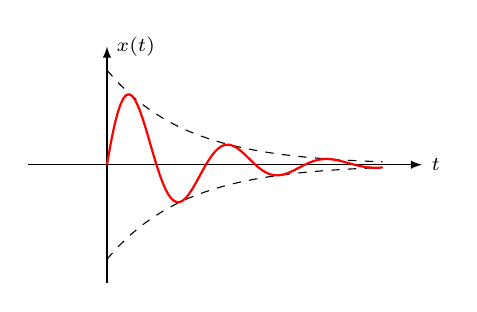
\begin{tikzpicture}[>=latex]
	\draw [->] (-1,0) -- (4,0) node [right] {\scriptsize \(t\)};
	\draw [->] (0,-1.5) -- (0,1.5) node [right] {\scriptsize \(x(t)\)};
	\draw [dashed, domain=0:3.5] plot(\x , {1.2*exp(-\x)});
	\draw [dashed, domain=0:3.5] plot(\x , {-1.2*exp(-\x)});
	\draw [thick , red , domain=0:3.5, samples = 100] plot(\x , {1.2*exp(-\x) * sin(5*\x r) });
\end{tikzpicture}

\end{document}
